\documentclass[12pt]{extarticle}
\usepackage[a4paper,margin=1in]{geometry}
\usepackage{amsmath}
\usepackage{graphicx}
\usepackage{float}
\usepackage{subcaption}
\usepackage{fontawesome}
\usepackage{amssymb}
\usepackage[colorlinks=true, linkcolor=blue, urlcolor=blue]{hyperref}
\newcommand{\thinking}{
\includegraphics[height=1.2em]{thinking.png}}
\newcommand{\allthebest}{
\includegraphics[height=7em]{all_the_best.png}}

\begin{document}
\begin{titlepage}
    \begin{center}
        
\includegraphics[width=0.3\textwidth]{iitb_logo.png}\\[1.5cm]
        {\LARGE \bfseries Blockchain Arena}\\
        \vspace{0.5cm}
        {\Large \bfseries Simulating Mining Wars and Network Attacks}\\
        \vspace{1cm}
        {\LARGE \bfseries Project 1}\\
        \vspace{0.5cm}
        {\Large \bfseries Simulation of a P2P Cryptocurrency Network}\\
        \vspace{1.5cm}
        {\Large \bf Release Date: June 13, 2025}\\
        \vspace{0.5cm}
        {\Large \bf Due Date: 23:59hrs, June 25, 2025}\\
        \vspace{3cm}
        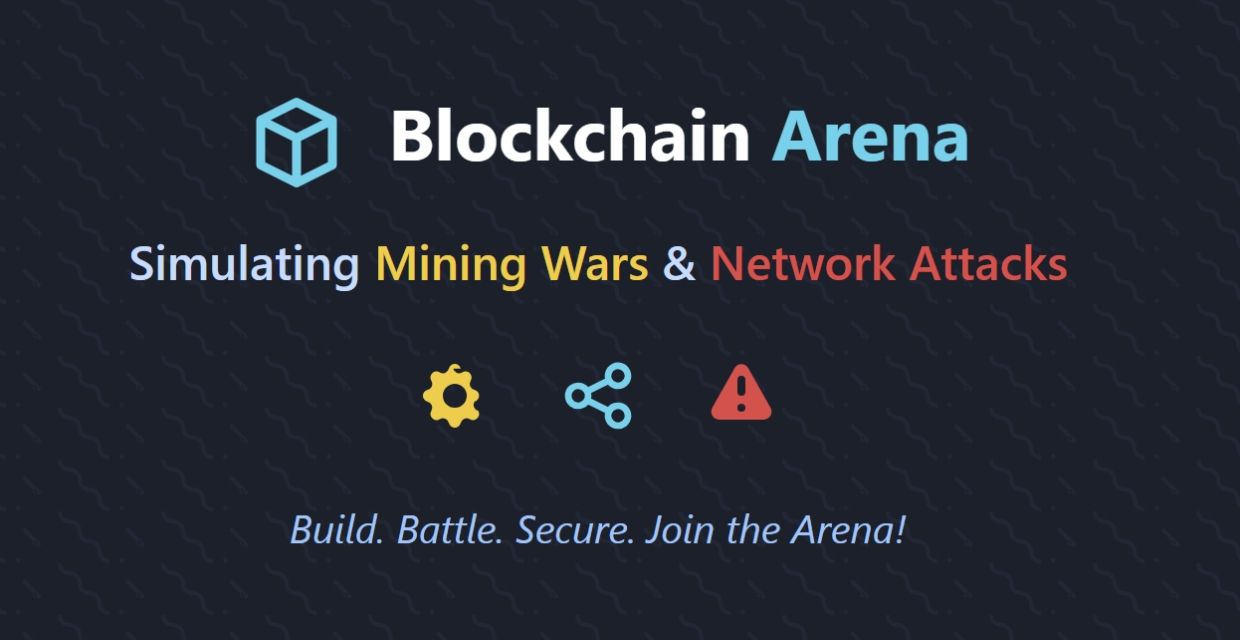
\includegraphics[width=0.9\textwidth]{blockchain_arena.jpeg}\\[1.5cm]
    \end{center}
\end{titlepage}

\section*{Objective}
In this assignment, you will build your own \textbf{discrete-event simulator} for a \textbf{P2P cryptocurrency network}. This simulation will be built upon your first assignment where you have created a P2P network topology.\\
\textbf{Discrete-Event Simulator}: It maintains an \textbf{event-queue} from which the earliest event is executed. This event may create further future events that get added to the queue. For example, an \texttt{send\_block} event in which one node sends a block to connected peers will create future events of \texttt{receive\_block} at its peers.
\subsection*{Suggestions}
\begin{itemize}
    \item I recommend using Python or C++ for this assignment. You can use any other programming language, but ensure that the code is well-structured and modular.
    \item If you include code from a publicly available source, it should be clearly mentioned in the comments. Don't copy-paste code from online GitHub repositories if available.
    \item Use of Generative AI tools like ChatGPT, Gemini, etc. is allowed for template code, but make sure to understand the code and modify it as per the requirements. \textbf{Don't} copy-paste code generated by these tools without understanding it.
\end{itemize}
\hrulefill
\section*{Network and Node Properties}
The cryptocurrency network must have the following properties:
\begin{enumerate}
    \item There are $n$ peers, each with a unique ID, where $n$ is a parameter set at the time of initiation of the network. Some of these nodes (say $z_0$ percent, where $z_0$ is a command line simulation parameter) are labeled \texttt{slow} and the others \texttt{fast}. In addition, some of these nodes (say $z_1$ percent, where $z_1$ is again a command line simulation parameter) are labeled \texttt{low CPU} and the others \texttt{high CPU}. We will use this classification below. \textbf{Tip:} Create a class \texttt{Peer} with required attributes.

    \item Each peer generates transactions randomly in time. The interarrival time between transactions generated by any peer is chosen from an exponential distribution whose \texttt{mean time} $(T_{tx})$ can be set as a parameter of the simulator.
          \begin{itemize}
              \item (Mention in report) What are the theoretical reasons of choosing the exponential distribution for interarrival time sampling?
          \end{itemize}
    \item Each transaction has the format: ``TxnID: $ID_x$ pays $ID_y$ C coins". You must ensure that C is less than or equal to the coins currently owned by $ID_x$ (ID of the peer that generates the transaction) before including it in a block. $ID_y$ should be the ID of any other peer in the network to which the transaction is destined ($ID_y$ should be chosen randomly). The size of each transaction is assumed to be 1 KB. \textbf{Tip:} Create a class \texttt{Transaction} with attributes like \texttt{TxnID}, \texttt{ID\_x}, \texttt{ID\_y}, \texttt{C} etc.

    \item \textbf{(Network Topology)} This is the same P2P network that you have created as part of the first assignment. The P2P network should satisfy the following properties:
          \begin{itemize}
              \item Each peer is randomly connected to between 3 and 6 other peers.
              \item The network is undirected and connected.
          \end{itemize}
          \textbf{Tip:} Use the \texttt{Network} class that you have implemented in the first assignment to represent the P2P network and maintain a list of peers.
    \item Simulate latencies $L_{ij}$ between pairs of peers $i$ and $j$ connected by a link. Latency is the time between which a message $m$ was transmitted from the sender $i$ and received by another node $j$. Choose the latency to be of the form $\rho_{ij} + |m|/c_{ij} + d_{ij}$, where $\rho_{ij}$ is a positive minimum value corresponding to the speed of light propagation delay, $|m|$ denotes the length of the message in bits, $c_{ij}$ is the link speed between $i$ and $j$ in bits per second, and $d_{ij}$ is the queuing delay at node $i$ to forward the message to node $j$. $d_{ij}$ is randomly chosen from an exponential distribution with mean $96kbits/c_{i,j}$. Note that $d_{i,j}$ must be randomly chosen for each message transmitted from $i$ to $j$. $\rho_{ij}$ can be chosen from a uniform distribution between 10ms and 500ms at the start of the simulation. $c_{ij}$ is set to 100 Mbps if both $i$ and $j$ are fast, and to 5 Mbps if either of the nodes is slow.
          \begin{itemize}
              \item (Mention in report) Why is the mean of $d_{ij}$ (queuing delay) inversely related to $c_{ij}$ (link speed)? Give justification for this choice.
          \end{itemize}

    \item A node forwards any transaction it receives from one peer to another connected peer, as long as it has not already sent the transaction to that peer and has not received it from that peer. This prevents transactions from circulating in endless loops (loop-less forwarding).
\end{enumerate}

\hrulefill

\section*{Simulating Proof-of-Work (PoW)}
\begin{enumerate}
    \setcounter{enumi}{6} % Start numbering from 7
    \item All nodes have the genesis block at the start of the simulation. Each block must have a unique ID, say BlkID (use a suitable method to generate unique block Id). Any peer, say peer $k$, maintains a tree of blocks as in bitcoin. When it receives a block from another peer, it validates all its transactions (no balance of any peer should go negative), and if the block is valid it adds the block to its tree.

          When a received block creates a new longest chain at peer $k$ (longer than the previous longest chain), say at time $t_k$, then we simulate PoW mining of a new block as follows. Peer $k$ forms a block at $t_k$ by selecting a subset of the transactions received so far and not included in any blocks in the longest chain. After forming a block, node $k$ generates a random variable $T_k$, at time $t_k$, as follows:

          Suppose the interarrival time between blocks on average is $I$ (for example, $I$ is 600 sec in Bitcoin), and node $k$ has fraction $h_k$ (where $0 < h_k < 1$) of the total hashing power. Then $T_k$ is drawn from an exponential distribution with mean equal to $I/h_k$. If peer $k$ is a high CPU node, then it is assumed to have 10 times higher hashing power than a low CPU node. (Note: ensure that the $\sum_k h_k = 1$ in the simulation).

          If peer $k$ has the same longest chain at time $t_k + T_k$ then it broadcasts a new block. (If it no longer has the same longest chain at $t_k + T_k$ then the event scheduled for mining a block at $t_k + T_k$ is terminated.) This block lists the BlkID of the last block in the longest received chain of the node and the list of transactions included in it. Once broadcast, the node starts creating a new block from this terminal block which is now the \texttt{longest\_chain\_tip}. The block is assumed to contribute \textbf{50} coins to $k$ (i.e. $ID_k$) as a mining fee, and this is included as a coinbase transaction ``TxnID: $ID_k$ mines 50 coins". On the contrary, if node $k$ receives the block from another node in the network, it validates all its transactions. Valid transactions are those where the sender has sufficient balance to perform the transaction. After validation, the node again starts block creation, as explained above.

          The block propagates in the network just like individual transactions. A block can have size at max 1 MB ($8 \times 10^6$ bits) and actual size depends on the number of transactions encapsulated in the block. An empty block (with no transactions besides the coinbase) is assumed to be of size 1KB. Ensure that you do not add too many transactions in the block such that the size of the block exceeds the maximum permitted size i.e. 1 MB. Make sure proper resolution of forks is done, i.e., the longest chain is always maintained.
          \begin{itemize}
              \item (Mention in report) The theoretical reason for choosing the exponential distribution for $T_k$ and the choice of its values set by you during experiments.
          \end{itemize}
          \textbf{Tip:} Create a \texttt{block} class to manage block creation, block validation, mining, etc.

    \item Each node maintains a tree of all blockchains heard since the start of the simulation. The node stores the time of arrival of every block in its tree. This information is written to a file at the end of the simulation.\\ \textbf{Tip:} Use a class \texttt{BlockchainTree} to manage the tree of blocks. The tree should have methods to add blocks, validate blocks, and find the longest chain.
\end{enumerate}
\hrulefill

\section*{Hint: How to build the Simulator? \thinking}
I recommend to build a centralized simulator around a single event queue. The simulator's core job is to process events from this queue in chronological order based on time.

To guide your design, consider the following tips:
\begin{itemize}
    \item Create a central \texttt{Simulator} class to manage the global time and the event queue.
    \item An \texttt{Event} class could represent different actions. Using an \texttt{enum} for event types (e.g., \texttt{GENERATE\_TRANSACTION}, \texttt{RECEIVE\_BLOCK}) is a good way to identify them.
    \item The main loop would dequeue the earliest event and dispatch it to the correct node that will handle the event based on its type.
    \item A key concept is that handling one event can create new, future events that are added back to the queue.  For example, a node receiving a block will then create future events for its peers to receive that same block.
\end{itemize}

\section*{Analysis and Experimentation}
Use an appropriate visualization tool to study the blockchain tree. Experiment with choosing different values for different parameters ($n, z_0, z_1, T_{tx}$, mean of $T_k$ etc.). Find the ratio of the number of blocks generated by each node in the Longest Chain of the tree to the total number of blocks it generates at the end of the simulation. How does this ratio vary depending on whether the node is fast, slow, low CPU, high CPU power etc.? How long are branches of the tree measured in number of blocks? Give detailed insights to explain your observations and findings in the report.
\section*{Submission Guidelines}
Submit the GitHub repository link containing the following files:
\begin{enumerate}
    \item Source code for simulator and visualization tool that you have used.
    \item \texttt{README.md} file with instructions for compiling and running.
    \item A report that includes the explnations as per the assignment, detailing your findings along with pictures of typical blockchain trees and appropriate insights.
\end{enumerate}
\textbf{Submission Link:} \href{https://docs.google.com/forms/d/e/1FAIpQLSf3PmpIGiE9gxEq83tuMBG4SozIBBrWrcAXwvg-zlrZ72bfVQ/viewform?usp=dialog}{Google Form for Submission}\\
\textbf{Deadline:} 23:59hrs, June 25, 2025.\\
\vspace{1cm}
\begin{center}
    \allthebest\\
    \textbf{Be patient and Enjoy building the simulator!}
\end{center}
\end{document}